\documentclass[letterpaper,12pt]{article}
\usepackage[utf8]{inputenc}

\usepackage{rotating}
\usepackage[top=1in, bottom=1in, left=1in, right=1in]{geometry}
\usepackage{graphicx}
\usepackage[numbers,square,sort&compress]{natbib}
\usepackage{setspace}
\usepackage[cdot,mediumqspace,]{SIunits}
\usepackage{hyperref}
\usepackage{mathtools}
\usepackage{url}
\usepackage{authblk}
\usepackage{placeins}
\usepackage{float}

\onehalfspacing
\title{Computational Physics Lab 10}
\author{Anita Bahmanyar}
\affil{\small {Student Number: 998909098}}
\date{November 14, 2014}

\usepackage{graphicx}

\renewcommand\thesubsection{\alph{subsection}}

\begin{document}

\maketitle

\section*{Q1}
The green box shows the boundary of the box so its easier to see that its not passing the boundary.

%figue a
\FloatBarrier
\begin{figure}[H]
\centering
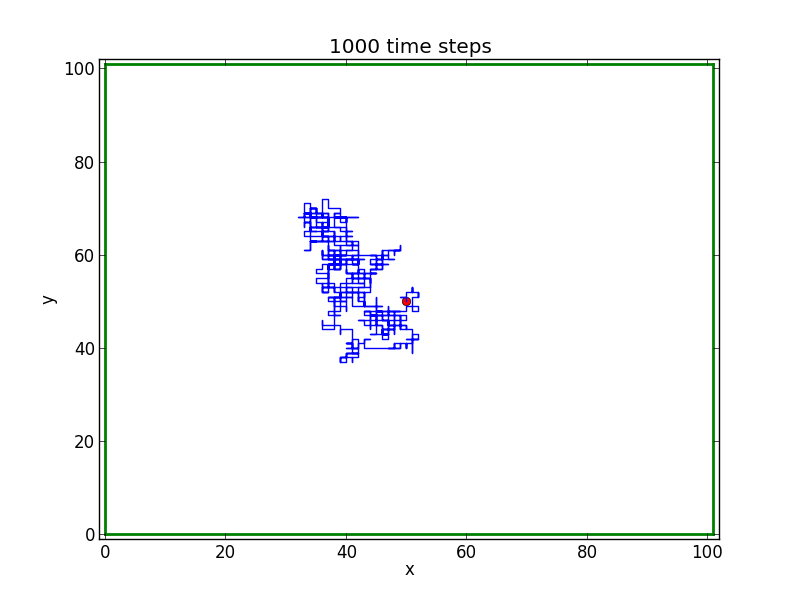
\includegraphics[scale=0.55]{q1a.png}
\caption{}
\end{figure}
\FloatBarrier

%figure b
\FloatBarrier
\begin{figure}[H]
\centering
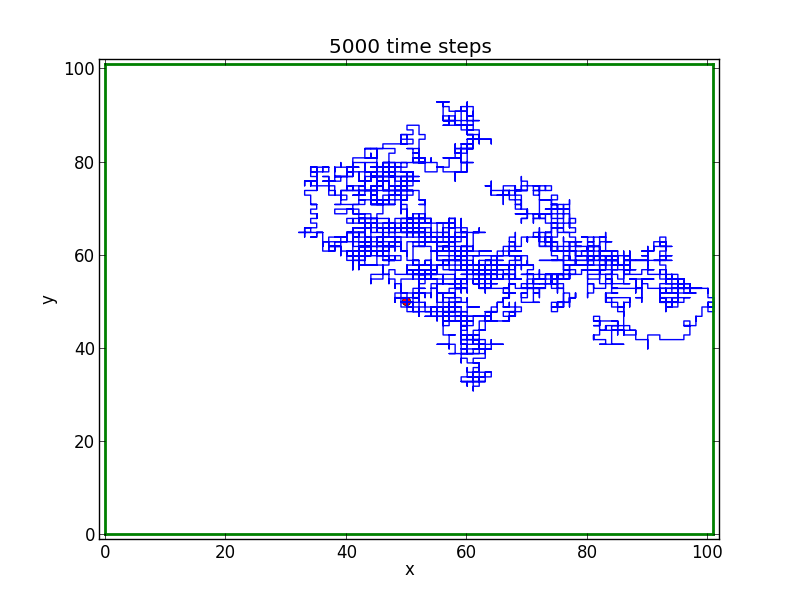
\includegraphics[scale=0.55]{q1b.png}
\caption{}
\end{figure}
\FloatBarrier


\section*{Q3}

\section*{Q4}
The integral value is 2.533376 $\pm$ 0.0508700209361.


\section*{Q6}

\FloatBarrier
\begin{figure}[H]
\centering
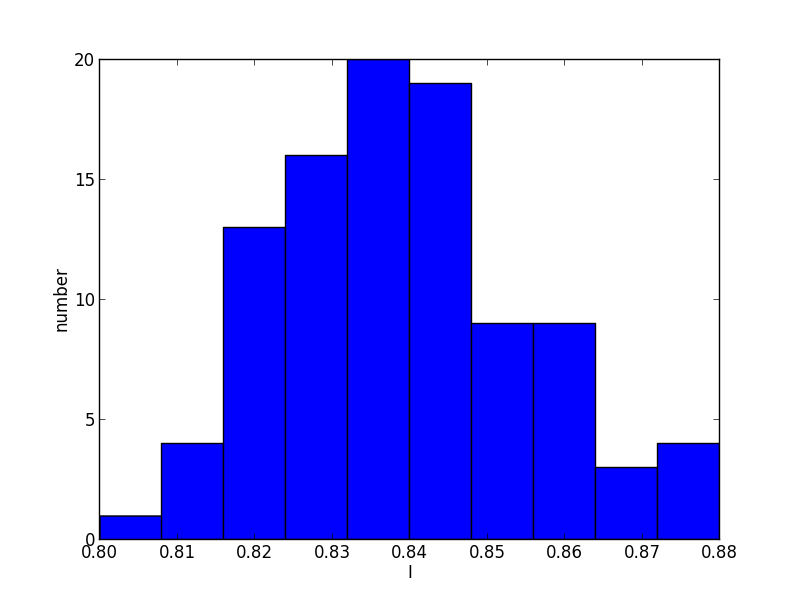
\includegraphics[scale=0.55]{q6.png}
\caption{}
\end{figure}
\FloatBarrier

\section*{Q7}

\FloatBarrier
\begin{figure}[H]
\centering
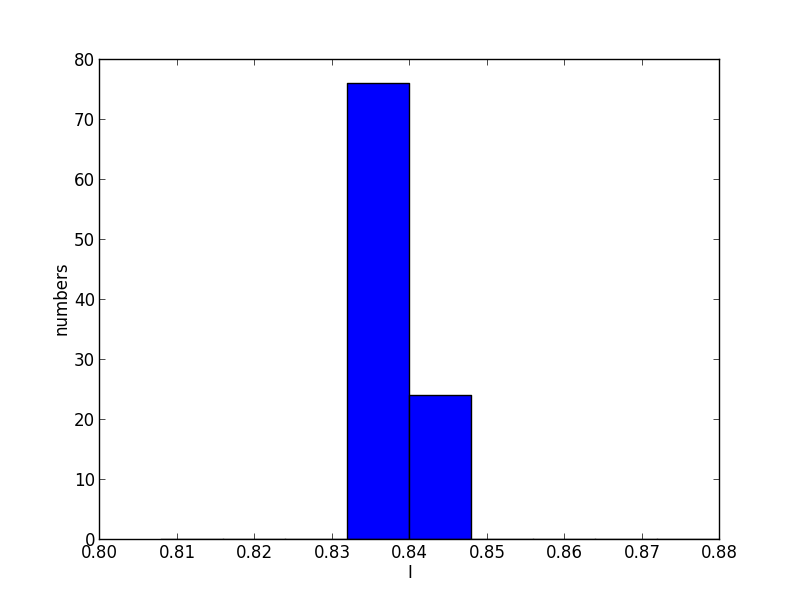
\includegraphics[scale=0.55]{q7.png}
\caption{}
\end{figure}
\FloatBarrier

As the histogram shows the method done in this question is much better than the method done in question 5 and 6, since the histogram has less spread in question 7, which means the value obtained is better.
\\In this question, I used the value of 2 for the $\int w$ by calculating it by hand. I also put the part in my code that calculates the integral of w using gaussian quadrature method and the value I got is 1.999 which is pretty close to the actual value, but using this value will introduce some error to the calculation of the integral.

\end{document}


